\documentclass[12pt]{elsart}
\usepackage{amsmath}
\usepackage{amssymb}
\usepackage[table]{xcolor}
\usepackage{tikz-qtree}
\usepackage{tikz}

%\vspace{10 mm}

\begin{document}

\pagestyle{empty}
\newpage

{\bf 1.} $sup_{min} = 60\% = 3$, $conf_{min} = 80\%$

{\bf (a)} Find all frequent  itemsets by following the Apriori Algorithm.

\begin{tabular}{|c|c|}
  \hline
  \multicolumn{2}{|c|}{$C_1$} \\
  \hline
  itemset & count \\ \hline
  \cellcolor{red} A & 1 \\ \hline
  \cellcolor{red} C & 2 \\ \hline
  \cellcolor{red} D & 1 \\ \hline
  E & 4 \\ \hline
  \cellcolor{red} I & 1 \\ \hline
  K & 5 \\ \hline
  M & 3 \\ \hline
  \cellcolor{red} N & 2 \\ \hline
  O & 3 \\ \hline
  \cellcolor{red} U & 1 \\ \hline
  \cellcolor{red} Y & 2 \\
  \hline
\end{tabular}
$\Rightarrow$
\begin{tabular}{|c|c|}
  \hline
  \multicolumn{2}{|c|}{$L_1$} \\
  \hline
  itemset & count \\ \hline
  E & 4 \\ \hline
  K & 5 \\ \hline
  M & 3 \\ \hline
  O & 3 \\
  \hline
\end{tabular}
$\Rightarrow$
\begin{tabular}{|c|c|}
  \hline
  \multicolumn{2}{|c|}{$C_2$} \\
  \hline
  itemset & count \\ \hline
  EK & 4 \\ \hline
  \cellcolor{red} EM & 2 \\ \hline
  EO & 3 \\ \hline
  KM & 3 \\ \hline
  KO & 3 \\ \hline
  \cellcolor{red} MO & 1 \\
  \hline
\end{tabular}
$\Rightarrow$
\begin{tabular}{|c|c|}
  \hline
  \multicolumn{2}{|c|}{$L_2$} \\
  \hline
  itemset & count \\ \hline
  EK & 4 \\ \hline
  EO & 3 \\ \hline
  KM & 3 \\ \hline
  KO & 3 \\
  \hline
\end{tabular}

$\Rightarrow$
\begin{tabular}{|c|c|}
  \hline
  \multicolumn{2}{|c|}{$L_3$} \\
  \hline
  itemset & count \\ \hline
  EKO & 3 \\
  \hline
\end{tabular}

{\bf (b)} Identify closed and maximal frequent itemsets.

\begin{tabular}{|c|c|}
  \hline
  closed & K, EK, KM \\ \hline
  maximal & KM, EKO \\
  \hline
\end{tabular}

\newpage

{\bf (c)} Draw the hash tree for candidate 2-itemsets, assuming that the hash function  will map A, E, M, Y to the left branch, C, I, N to the center branch, and D, K, O, U to the right branch. (Circles are empty leaf nodes, squares are internal hash table nodes)

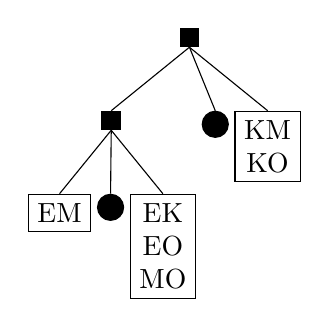
\begin{tikzpicture}
  \tikzset{every tree node/.style={align=center,anchor=north}}
  \Tree [.\node [draw,fill] {}; [.\node [draw,fill] {}; [.\node [draw] {EM}; ]
                                                        [.\node [circle,draw,fill] {}; ]
                                                        [.\node [draw] {EK\\EO\\MO}; ] ]
                                [.\node [circle,draw,fill] {}; ]
                                [.\node [draw] {KM\\KO}; ] ]
\end{tikzpicture}

{\bf (d)} Identify the hash tree nodes visited when counting the support of 2-itemsets for transaction T400. (Red means node was visited)

T400 $\Rightarrow$ \{M, U, C, K, Y\} $\Rightarrow$ \{C, K, M, U, Y\}

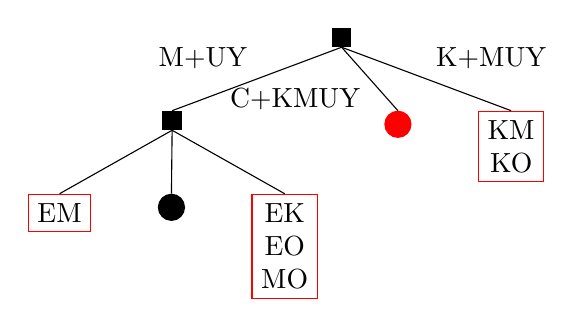
\begin{tikzpicture}[sibling distance=24pt]
  \tikzset{every tree node/.style={align=center,anchor=north}}
    \Tree [.\node [draw,fill] {}; \edge node[auto=right]{M+UY}; [.\node [draw,fill] {}; [.\node [draw=red] {EM}; ]
                                                          [.\node [circle,draw,fill] {}; ]
                                                          [.\node [draw=red] {EK\\EO\\MO}; ] ]
                                  \edge node[auto=right]{C+KMUY}; [.\node [circle,draw=red,fill=red] {}; ]
                                  \edge node[auto=left]{K+MUY}; [.\node [draw=red] {KM\\KO}; ] ]
\end{tikzpicture}

{\bf 2.} Let $sup_{min} = 60\% = 3$ and $conf_{min} = 80\%$. Find all frequent itemsets by following the FP-growth algorithm.

{\bf (a)} Find the F-list and draw the FP-tree.

\verb|F-list          F-tree|

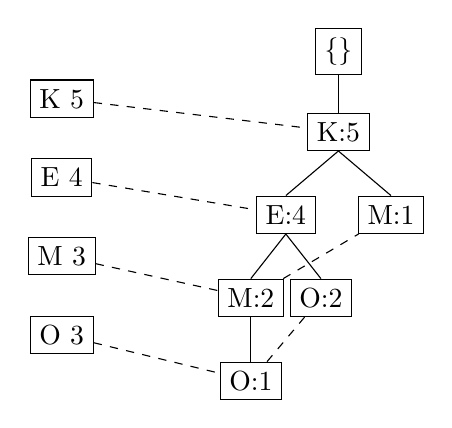
\begin{tikzpicture}
  \node [draw](O) at (0,0) {O 3};
  \node [draw](M) at (0,1) {M 3};
  \node [draw](E) at (0,2) {E 4};
  \node [draw](K) at (0,3) {K 5};
  \begin{scope}[xshift=100,yshift=100]
  \Tree [.\node [draw] {\{\}}; [.\node [draw](K1){K:5}; 
                                 [.\node(E1)[draw] {E:4};
                                   [.\node(M1)[draw] {M:2}; \node(O1)[draw] {O:1}; ]
                                   [.\node(O2)[draw] {O:2}; ] ]
                                 [.\node(M2)[draw] {M:1}; ] ] ]
  \end{scope}
  \begin{scope}[dashed]
    \draw (O)--(O1);
    \draw (O1)--(O2);
    \draw (M)--(M1);
    \draw (M1)--(M2);
    \draw (E)--(E1);
    \draw (K)--(K1);
  \end{scope}
\end{tikzpicture}

\newpage

{\bf (b)} For each projected database, list all frequent itemsets that can be enumerated from the database. (Asked professor, show conditional base and conditional tree for each)

prefix {\bf O}:
\begin{tabular}{|c|c|}
  \multicolumn{2}{c}{conditional bases} \\ \hline
  prefix & count \\ \hline
  KEM & 1 \\ \hline
  KE & 2 \\
  \hline
\end{tabular}
$\Rightarrow$
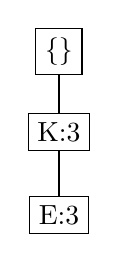
\begin{tikzpicture}
  \Tree [.\node [draw] {\{\}}; [.\node [draw] {K:3}; [.\node [draw] {E:3}; ] ] ]
\end{tikzpicture}
$\Rightarrow$
\begin{tabular}{|c|c|}
  \multicolumn{2}{c}{frequent patterns} \\ \hline
  pattern & count \\ \hline
  O & 3 \\ \hline
  KO & 3 \\ \hline
  EO & 3 \\ \hline
  KEO & 3 \\
  \hline
\end{tabular}

prefix {\bf M}:
\begin{tabular}{|c|c|}
  \multicolumn{2}{c}{conditional bases} \\ \hline
  prefix & count \\ \hline
  KE & 2 \\ \hline
  K & 1 \\
  \hline
\end{tabular}
$\Rightarrow$
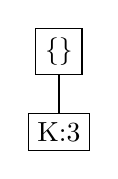
\begin{tikzpicture}
\Tree [.\node [draw] {\{\}}; [.\node [draw] {K:3}; ] ]
\end{tikzpicture}
$\Rightarrow$
\begin{tabular}{|c|c|}
  \multicolumn{2}{c}{frequent patterns} \\ \hline
  pattern & count \\ \hline
  M & 3 \\ \hline
  KM & 3 \\
  \hline
\end{tabular}

prefix {\bf E}:
\begin{tabular}{|c|c|}
  \multicolumn{2}{c}{conditional bases} \\ \hline
  prefix & count \\ \hline
  K & 4 \\
  \hline
\end{tabular}
$\Rightarrow$
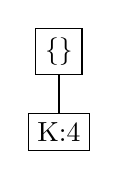
\begin{tikzpicture}
\Tree [.\node [draw] {\{\}}; [.\node [draw] {K:4}; ] ]
\end{tikzpicture}
$\Rightarrow$
\begin{tabular}{|c|c|}
  \multicolumn{2}{c}{frequent patterns} \\ \hline
  pattern & count \\ \hline
  E & 4 \\ \hline
  KE & 4 \\
  \hline
\end{tabular}

prefix {\bf K}:
\begin{tabular}{|c|c|}
  \multicolumn{2}{c}{conditional bases} \\ \hline
  prefix & count \\ \hline
    &  \\
  \hline
\end{tabular}
$\Rightarrow$

\begin{tikzpicture}
\Tree [.\node [draw] {\{\}}; ]
\end{tikzpicture}
$\Rightarrow$
\begin{tabular}{|c|c|}
  \multicolumn{2}{c}{frequent patterns} \\ \hline
  pattern & count \\ \hline
  K & 5 \\
  \hline
\end{tabular}

{\bf 3.} Find all association rules.

{\bf (a)} Identify all strong association rules.

{\bf (b)} Compute the lift measure for each strong association rule. (List both a and b together)

$1 buys(E), buys(K) \Rightarrow buys(O)[60\%, 75\%]$ $lift=1.25$ \\
$2 buys(E), buys(O) \Rightarrow buys(K)[60\%, 100\%]$ $lift=1$ \\
$3 buys(K), buys(O) \Rightarrow buys(E)[60\%, 100\%]$ $lift=1.25$ \\
$4 buys(E) \Rightarrow buys(K), buys(O)[60\%, 75\%]$ $lift=1.25$ \\
$5 buys(K) \Rightarrow buys(E), buys(O)[60\%, 60\%]$ $lift=1$ \\
$6 buys(O) \Rightarrow buys(E), buys(K)[60\%, 100\%]$ $lift=1.25$ \\
$7 buys(E) \Rightarrow buys(K)[80\%, 100\%]$ $lift=1$ \\
$8 buys(K) \Rightarrow buys(E)[80\%, 80\%]$ $lift=1$ \\
$9 buys(E) \Rightarrow buys(O)[60\%, 75\%]$ $lift=1.25$ \\
$10 buys(O) \Rightarrow buys(E)[60\%, 100\%]$ $lift=1.25$ \\
$11 buys(K) \Rightarrow buys(M)[60\%, 60\%]$ $lift=1$ \\
$12 buys(M) \Rightarrow buys(K)[60\%, 100\%]$ $lift=1$ \\
$13 buys(K) \Rightarrow buys(O)[60\%, 80\%]$ $lift=1$ \\
$14 buys(O) \Rightarrow buys(K)[60\%, 100\%]$ $lift=1$ \\

{\bf 4.} Convert the transaction data table into an hwk02.arff file, in which each item is a column
with either a value t or ? (that is, with a type {t}). Use Weka Explore to load the data, and run the Aproiri and FPGrowth algorithms to learn interesting association rules. Do it for at least three sets of minimum support and confidence. For each algorithm, report the following items.

{\bf (a)} The commands used to run the learning tasks (Labeled as 'Scheme' in the output)

{\bf (b)} The output from the runs

{\bf Apriori}:

\begin{verbatim}
1.
=== Run information ===

Scheme:       weka.associations.Apriori -I -N 20 -T 0 -C 0.8 -D 0.2 -U 1.0 -M 0.6 -S -1.0 -c -1
Relation:     hwk02
Instances:    5
Attributes:   11
A
C
D
E
I
K
M
N
O
U
Y
=== Associator model (full training set) ===


Apriori
=======

Minimum support: 0.6 (3 instances)
Minimum metric <confidence>: 0.8
Number of cycles performed: 3

Generated sets of large itemsets:

Size of set of large itemsets L(1): 4

Large Itemsets L(1):
E=t 4
K=t 5
M=t 3
O=t 3

Size of set of large itemsets L(2): 4

Large Itemsets L(2):
E=t K=t 4
E=t O=t 3
K=t M=t 3
K=t O=t 3

Size of set of large itemsets L(3): 1

Large Itemsets L(3):
E=t K=t O=t 3

Best rules found:

1. E=t 4 ==> K=t 4    <conf:(1)> lift:(1) lev:(0) [0] conv:(0)
2. O=t 3 ==> E=t 3    <conf:(1)> lift:(1.25) lev:(0.12) [0] conv:(0.6)
3. M=t 3 ==> K=t 3    <conf:(1)> lift:(1) lev:(0) [0] conv:(0)
4. O=t 3 ==> K=t 3    <conf:(1)> lift:(1) lev:(0) [0] conv:(0)
5. K=t O=t 3 ==> E=t 3    <conf:(1)> lift:(1.25) lev:(0.12) [0] conv:(0.6)
6. E=t O=t 3 ==> K=t 3    <conf:(1)> lift:(1) lev:(0) [0] conv:(0)
7. O=t 3 ==> E=t K=t 3    <conf:(1)> lift:(1.25) lev:(0.12) [0] conv:(0.6)
8. K=t 5 ==> E=t 4    <conf:(0.8)> lift:(1) lev:(0) [0] conv:(0.5)

2.
=== Run information ===

Scheme:       weka.associations.Apriori -I -N 50 -T 0 -C 0.9 -D 0.25 -U 1.0 -M 0.5 -S -1.0 -c -1
Relation:     hwk02
Instances:    5
Attributes:   11
A
C
D
E
I
K
M
N
O
U
Y
=== Associator model (full training set) ===


Apriori
=======

Minimum support: 0.5 (3 instances)
Minimum metric <confidence>: 0.9
Number of cycles performed: 2

Generated sets of large itemsets:

Size of set of large itemsets L(1): 4

Large Itemsets L(1):
E=t 4
K=t 5
M=t 3
O=t 3

Size of set of large itemsets L(2): 4

Large Itemsets L(2):
E=t K=t 4
E=t O=t 3
K=t M=t 3
K=t O=t 3

Size of set of large itemsets L(3): 1

Large Itemsets L(3):
E=t K=t O=t 3

Best rules found:

1. E=t 4 ==> K=t 4    <conf:(1)> lift:(1) lev:(0) [0] conv:(0)
2. O=t 3 ==> E=t 3    <conf:(1)> lift:(1.25) lev:(0.12) [0] conv:(0.6)
3. M=t 3 ==> K=t 3    <conf:(1)> lift:(1) lev:(0) [0] conv:(0)
4. O=t 3 ==> K=t 3    <conf:(1)> lift:(1) lev:(0) [0] conv:(0)
5. K=t O=t 3 ==> E=t 3    <conf:(1)> lift:(1.25) lev:(0.12) [0] conv:(0.6)
6. E=t O=t 3 ==> K=t 3    <conf:(1)> lift:(1) lev:(0) [0] conv:(0)
7. O=t 3 ==> E=t K=t 3    <conf:(1)> lift:(1.25) lev:(0.12) [0] conv:(0.6)

3.
=== Run information ===

Scheme:       weka.associations.Apriori -I -N 50 -T 0 -C 0.7 -D 0.1 -U 1.0 -M 0.4 -S -1.0 -c -1
Relation:     hwk02
Instances:    5
Attributes:   11
A
C
D
E
I
K
M
N
O
U
Y
=== Associator model (full training set) ===


Apriori
=======

Minimum support: 0.4 (2 instances)
Minimum metric <confidence>: 0.7
Number of cycles performed: 7

Generated sets of large itemsets:

Size of set of large itemsets L(1): 7

Large Itemsets L(1):
C=t 2
E=t 4
K=t 5
M=t 3
N=t 2
O=t 3
Y=t 2

Size of set of large itemsets L(2): 10

Large Itemsets L(2):
C=t K=t 2
E=t K=t 4
E=t M=t 2
E=t N=t 2
E=t O=t 3
K=t M=t 3
K=t N=t 2
K=t O=t 3
K=t Y=t 2
N=t O=t 2

Size of set of large itemsets L(3): 5

Large Itemsets L(3):
E=t K=t M=t 2
E=t K=t N=t 2
E=t K=t O=t 3
E=t N=t O=t 2
K=t N=t O=t 2

Size of set of large itemsets L(4): 1

Large Itemsets L(4):
E=t K=t N=t O=t 2

Best rules found:

1. E=t 4 ==> K=t 4    <conf:(1)> lift:(1) lev:(0) [0] conv:(0)
2. O=t 3 ==> E=t 3    <conf:(1)> lift:(1.25) lev:(0.12) [0] conv:(0.6)
3. M=t 3 ==> K=t 3    <conf:(1)> lift:(1) lev:(0) [0] conv:(0)
4. O=t 3 ==> K=t 3    <conf:(1)> lift:(1) lev:(0) [0] conv:(0)
5. K=t O=t 3 ==> E=t 3    <conf:(1)> lift:(1.25) lev:(0.12) [0] conv:(0.6)
6. E=t O=t 3 ==> K=t 3    <conf:(1)> lift:(1) lev:(0) [0] conv:(0)
7. O=t 3 ==> E=t K=t 3    <conf:(1)> lift:(1.25) lev:(0.12) [0] conv:(0.6)
8. C=t 2 ==> K=t 2    <conf:(1)> lift:(1) lev:(0) [0] conv:(0)
9. N=t 2 ==> E=t 2    <conf:(1)> lift:(1.25) lev:(0.08) [0] conv:(0.4)
10. N=t 2 ==> K=t 2    <conf:(1)> lift:(1) lev:(0) [0] conv:(0)
11. Y=t 2 ==> K=t 2    <conf:(1)> lift:(1) lev:(0) [0] conv:(0)
12. N=t 2 ==> O=t 2    <conf:(1)> lift:(1.67) lev:(0.16) [0] conv:(0.8)
13. E=t M=t 2 ==> K=t 2    <conf:(1)> lift:(1) lev:(0) [0] conv:(0)
14. K=t N=t 2 ==> E=t 2    <conf:(1)> lift:(1.25) lev:(0.08) [0] conv:(0.4)
15. E=t N=t 2 ==> K=t 2    <conf:(1)> lift:(1) lev:(0) [0] conv:(0)
16. N=t 2 ==> E=t K=t 2    <conf:(1)> lift:(1.25) lev:(0.08) [0] conv:(0.4)
17. N=t O=t 2 ==> E=t 2    <conf:(1)> lift:(1.25) lev:(0.08) [0] conv:(0.4)
18. E=t N=t 2 ==> O=t 2    <conf:(1)> lift:(1.67) lev:(0.16) [0] conv:(0.8)
19. N=t 2 ==> E=t O=t 2    <conf:(1)> lift:(1.67) lev:(0.16) [0] conv:(0.8)
20. N=t O=t 2 ==> K=t 2    <conf:(1)> lift:(1) lev:(0) [0] conv:(0)
21. K=t N=t 2 ==> O=t 2    <conf:(1)> lift:(1.67) lev:(0.16) [0] conv:(0.8)
22. N=t 2 ==> K=t O=t 2    <conf:(1)> lift:(1.67) lev:(0.16) [0] conv:(0.8)
23. K=t N=t O=t 2 ==> E=t 2    <conf:(1)> lift:(1.25) lev:(0.08) [0] conv:(0.4)
24. E=t N=t O=t 2 ==> K=t 2    <conf:(1)> lift:(1) lev:(0) [0] conv:(0)
25. E=t K=t N=t 2 ==> O=t 2    <conf:(1)> lift:(1.67) lev:(0.16) [0] conv:(0.8)
26. N=t O=t 2 ==> E=t K=t 2    <conf:(1)> lift:(1.25) lev:(0.08) [0] conv:(0.4)
27. K=t N=t 2 ==> E=t O=t 2    <conf:(1)> lift:(1.67) lev:(0.16) [0] conv:(0.8)
28. E=t N=t 2 ==> K=t O=t 2    <conf:(1)> lift:(1.67) lev:(0.16) [0] conv:(0.8)
29. N=t 2 ==> E=t K=t O=t 2    <conf:(1)> lift:(1.67) lev:(0.16) [0] conv:(0.8)
30. K=t 5 ==> E=t 4    <conf:(0.8)> lift:(1) lev:(0) [0] conv:(0.5)
31. E=t 4 ==> O=t 3    <conf:(0.75)> lift:(1.25) lev:(0.12) [0] conv:(0.8)
32. E=t K=t 4 ==> O=t 3    <conf:(0.75)> lift:(1.25) lev:(0.12) [0] conv:(0.8)
33. E=t 4 ==> K=t O=t 3    <conf:(0.75)> lift:(1.25) lev:(0.12) [0] conv:(0.8)
\end{verbatim}

{\bf FP-Growth}:

\begin{verbatim}
1.
=== Run information ===

Scheme:       weka.associations.FPGrowth -P 2 -I -1 -N 50 -T 0 -C 0.6 -D 0.05 -U 1.0 -M 0.8 -S
Relation:     hwk02
Instances:    5
Attributes:   11
A
C
D
E
I
K
M
N
O
U
Y
=== Associator model (full training set) ===

FPGrowth found 2 rules

1. [E=t]: 4 ==> [K=t]: 4   <conf:(1)> lift:(1) lev:(0) conv:(0) 
2. [K=t]: 5 ==> [E=t]: 4   <conf:(0.8)> lift:(1) lev:(0) conv:(0.5) 

2.
=== Run information ===

Scheme:       weka.associations.FPGrowth -P 2 -I -1 -N 50 -T 0 -C 0.6 -D 0.05 -U 1.0 -M 0.4 -S
Relation:     hwk02
Instances:    5
Attributes:   11
A
C
D
E
I
K
M
N
O
U
Y
=== Associator model (full training set) ===

FPGrowth found 48 rules

1. [E=t]: 4 ==> [K=t]: 4   <conf:(1)> lift:(1) lev:(0) conv:(0) 
2. [O=t]: 3 ==> [K=t]: 3   <conf:(1)> lift:(1) lev:(0) conv:(0) 
3. [M=t]: 3 ==> [K=t]: 3   <conf:(1)> lift:(1) lev:(0) conv:(0) 
4. [Y=t]: 2 ==> [K=t]: 2   <conf:(1)> lift:(1) lev:(0) conv:(0) 
5. [N=t]: 2 ==> [K=t]: 2   <conf:(1)> lift:(1) lev:(0) conv:(0) 
6. [C=t]: 2 ==> [K=t]: 2   <conf:(1)> lift:(1) lev:(0) conv:(0) 
7. [O=t]: 3 ==> [E=t]: 3   <conf:(1)> lift:(1.25) lev:(0.12) conv:(0.6) 
8. [N=t]: 2 ==> [E=t]: 2   <conf:(1)> lift:(1.25) lev:(0.08) conv:(0.4) 
9. [N=t]: 2 ==> [O=t]: 2   <conf:(1)> lift:(1.67) lev:(0.16) conv:(0.8) 
10. [O=t]: 3 ==> [K=t, E=t]: 3   <conf:(1)> lift:(1.25) lev:(0.12) conv:(0.6) 
11. [K=t, O=t]: 3 ==> [E=t]: 3   <conf:(1)> lift:(1.25) lev:(0.12) conv:(0.6) 
12. [E=t, O=t]: 3 ==> [K=t]: 3   <conf:(1)> lift:(1) lev:(0) conv:(0) 
13. [E=t, M=t]: 2 ==> [K=t]: 2   <conf:(1)> lift:(1) lev:(0) conv:(0) 
14. [N=t]: 2 ==> [K=t, E=t]: 2   <conf:(1)> lift:(1.25) lev:(0.08) conv:(0.4) 
15. [K=t, N=t]: 2 ==> [E=t]: 2   <conf:(1)> lift:(1.25) lev:(0.08) conv:(0.4) 
16. [E=t, N=t]: 2 ==> [K=t]: 2   <conf:(1)> lift:(1) lev:(0) conv:(0) 
17. [N=t]: 2 ==> [K=t, O=t]: 2   <conf:(1)> lift:(1.67) lev:(0.16) conv:(0.8) 
18. [K=t, N=t]: 2 ==> [O=t]: 2   <conf:(1)> lift:(1.67) lev:(0.16) conv:(0.8) 
19. [O=t, N=t]: 2 ==> [K=t]: 2   <conf:(1)> lift:(1) lev:(0) conv:(0) 
20. [N=t]: 2 ==> [E=t, O=t]: 2   <conf:(1)> lift:(1.67) lev:(0.16) conv:(0.8) 
21. [E=t, N=t]: 2 ==> [O=t]: 2   <conf:(1)> lift:(1.67) lev:(0.16) conv:(0.8) 
22. [O=t, N=t]: 2 ==> [E=t]: 2   <conf:(1)> lift:(1.25) lev:(0.08) conv:(0.4) 
23. [N=t]: 2 ==> [K=t, E=t, O=t]: 2   <conf:(1)> lift:(1.67) lev:(0.16) conv:(0.8) 
24. [K=t, N=t]: 2 ==> [E=t, O=t]: 2   <conf:(1)> lift:(1.67) lev:(0.16) conv:(0.8) 
25. [E=t, N=t]: 2 ==> [K=t, O=t]: 2   <conf:(1)> lift:(1.67) lev:(0.16) conv:(0.8) 
26. [K=t, E=t, N=t]: 2 ==> [O=t]: 2   <conf:(1)> lift:(1.67) lev:(0.16) conv:(0.8) 
27. [O=t, N=t]: 2 ==> [K=t, E=t]: 2   <conf:(1)> lift:(1.25) lev:(0.08) conv:(0.4) 
28. [K=t, O=t, N=t]: 2 ==> [E=t]: 2   <conf:(1)> lift:(1.25) lev:(0.08) conv:(0.4) 
29. [E=t, O=t, N=t]: 2 ==> [K=t]: 2   <conf:(1)> lift:(1) lev:(0) conv:(0) 
30. [K=t]: 5 ==> [E=t]: 4   <conf:(0.8)> lift:(1) lev:(0) conv:(0.5) 
31. [E=t]: 4 ==> [O=t]: 3   <conf:(0.75)> lift:(1.25) lev:(0.12) conv:(0.8) 
32. [E=t]: 4 ==> [K=t, O=t]: 3   <conf:(0.75)> lift:(1.25) lev:(0.12) conv:(0.8) 
33. [K=t, E=t]: 4 ==> [O=t]: 3   <conf:(0.75)> lift:(1.25) lev:(0.12) conv:(0.8) 
34. [M=t]: 3 ==> [E=t]: 2   <conf:(0.67)> lift:(0.83) lev:(-0.08) conv:(0.3) 
35. [O=t]: 3 ==> [N=t]: 2   <conf:(0.67)> lift:(1.67) lev:(0.16) conv:(0.9) 
36. [M=t]: 3 ==> [K=t, E=t]: 2   <conf:(0.67)> lift:(0.83) lev:(-0.08) conv:(0.3) 
37. [K=t, M=t]: 3 ==> [E=t]: 2   <conf:(0.67)> lift:(0.83) lev:(-0.08) conv:(0.3) 
38. [O=t]: 3 ==> [K=t, N=t]: 2   <conf:(0.67)> lift:(1.67) lev:(0.16) conv:(0.9) 
39. [K=t, O=t]: 3 ==> [N=t]: 2   <conf:(0.67)> lift:(1.67) lev:(0.16) conv:(0.9) 
40. [O=t]: 3 ==> [E=t, N=t]: 2   <conf:(0.67)> lift:(1.67) lev:(0.16) conv:(0.9) 
41. [E=t, O=t]: 3 ==> [N=t]: 2   <conf:(0.67)> lift:(1.67) lev:(0.16) conv:(0.9) 
42. [O=t]: 3 ==> [K=t, E=t, N=t]: 2   <conf:(0.67)> lift:(1.67) lev:(0.16) conv:(0.9) 
43. [K=t, O=t]: 3 ==> [E=t, N=t]: 2   <conf:(0.67)> lift:(1.67) lev:(0.16) conv:(0.9) 
44. [E=t, O=t]: 3 ==> [K=t, N=t]: 2   <conf:(0.67)> lift:(1.67) lev:(0.16) conv:(0.9) 
45. [K=t, E=t, O=t]: 3 ==> [N=t]: 2   <conf:(0.67)> lift:(1.67) lev:(0.16) conv:(0.9) 
46. [K=t]: 5 ==> [O=t]: 3   <conf:(0.6)> lift:(1) lev:(0) conv:(0.67) 
47. [K=t]: 5 ==> [M=t]: 3   <conf:(0.6)> lift:(1) lev:(0) conv:(0.67) 
48. [K=t]: 5 ==> [E=t, O=t]: 3   <conf:(0.6)> lift:(1) lev:(0) conv:(0.67)

3.
=== Run information ===

Scheme:       weka.associations.FPGrowth -P 2 -I -1 -N 50 -T 0 -C 0.9 -D 0.05 -U 1.0 -M 0.6 -S
Relation:     hwk02
Instances:    5
Attributes:   11
A
C
D
E
I
K
M
N
O
U
Y
=== Associator model (full training set) ===

FPGrowth found 7 rules

1. [E=t]: 4 ==> [K=t]: 4   <conf:(1)> lift:(1) lev:(0) conv:(0) 
2. [O=t]: 3 ==> [K=t]: 3   <conf:(1)> lift:(1) lev:(0) conv:(0) 
3. [M=t]: 3 ==> [K=t]: 3   <conf:(1)> lift:(1) lev:(0) conv:(0) 
4. [O=t]: 3 ==> [E=t]: 3   <conf:(1)> lift:(1.25) lev:(0.12) conv:(0.6) 
5. [O=t]: 3 ==> [K=t, E=t]: 3   <conf:(1)> lift:(1.25) lev:(0.12) conv:(0.6) 
6. [K=t, O=t]: 3 ==> [E=t]: 3   <conf:(1)> lift:(1.25) lev:(0.12) conv:(0.6) 
7. [E=t, O=t]: 3 ==> [K=t]: 3   <conf:(1)> lift:(1) lev:(0) conv:(0)
\end{verbatim}

\end{document}